%!TeX root=../sensetop.tex
\chapter[Chapter \thechapter]{}
\lettrine[lines=4,lraise=0.3]{E}{linor} saw, with great uneasiness the low spirits of her friend. His visit afforded her but a very partial satisfaction, while his own enjoyment in it appeared so imperfect. It was evident that he was unhappy; she wished it were equally evident that he still distinguished her by the same affection which once she had felt no doubt of inspiring; but hitherto the continuance of his preference seemed very uncertain; and the reservedness of his manner towards her contradicted one moment what a more animated look had intimated the preceding one.

He joined her and Marianne in the breakfast-room the next morning before the others were down; and Marianne, who was always eager to promote their happiness as far as she could, soon left them to themselves. But before she was half way upstairs she heard the parlour door open, and, turning round, was astonished to see Edward himself come out.

»I am going into the village to see my horses,« said he, »as you are not yet ready for breakfast; I shall be back again presently.«

Edward returned to them with fresh admiration of the surrounding country; in his walk to the village, he had seen many parts of the valley to advantage; and the village itself, in a much higher situation than the cottage, afforded a general view of the whole, which had exceedingly pleased him. This was a subject which ensured Marianne’s attention, and she was beginning to describe her own admiration of these scenes, and to question him more minutely on the objects that had particularly struck him, when Edward interrupted her by saying, »You must not enquire too far, Marianne—remember I have no knowledge in the picturesque, and I shall offend you by my ignorance and want of taste if we come to particulars. I shall call hills steep, which ought to be bold; surfaces strange and uncouth, which ought to be irregular and rugged; and distant objects out of sight, which ought only to be indistinct through the soft medium of a hazy atmosphere. You must be satisfied with such admiration as I can honestly give. I call it a very fine country—the hills are steep, the woods seem full of fine timber, and the valley looks comfortable and snug—with rich meadows and several neat farm houses scattered here and there. It exactly answers my idea of a fine country, because it unites beauty with utility—and I dare say it is a picturesque one too, because you admire it; I can easily believe it to be full of rocks and promontories, grey moss and brush wood, but these are all lost on me. I know nothing of the picturesque.«

»I am afraid it is but too true,« said Marianne; »but why should you boast of it?«

»I suspect,« said Elinor, »that to avoid one kind of affectation, Edward here falls into another. Because he believes many people pretend to more admiration of the beauties of nature than they really feel, and is disgusted with such pretensions, he affects greater indifference and less discrimination in viewing them himself than he possesses. He is fastidious and will have an affectation of his own.«

»It is very true,« said Marianne, »that admiration of landscape scenery is become a mere jargon. Every body pretends to feel and tries to describe with the taste and elegance of him who first defined what picturesque beauty was. I detest jargon of every kind, and sometimes I have kept my feelings to myself, because I could find no language to describe them in but what was worn and hackneyed out of all sense and meaning.«

»I am convinced,« said Edward, »that you really feel all the delight in a fine prospect which you profess to feel. But, in return, your sister must allow me to feel no more than I profess. I like a fine prospect, but not on picturesque principles. I do not like crooked, twisted, blasted trees. I admire them much more if they are tall, straight, and flourishing. I do not like ruined, tattered cottages. I am not fond of nettles or thistles, or heath blossoms. I have more pleasure in a snug farm-house than a watch-tower—and a troop of tidy, happy villagers please me better than the finest banditti in the world.«

Marianne looked with amazement at Edward, with compassion at her sister. Elinor only laughed.

The subject was continued no farther; and Marianne remained thoughtfully silent, till a new object suddenly engaged her attention. She was sitting by Edward, and in taking his tea from Mrs Dashwood, his hand passed so directly before her, as to make a ring, with a plait of hair in the centre, very conspicuous on one of his fingers.

»I never saw you wear a ring before, Edward,« she cried. »Is that Fanny’s hair? I remember her promising to give you some. But I should have thought her hair had been darker.«

Marianne spoke inconsiderately what she really felt—but when she saw how much she had pained Edward, her own vexation at her want of thought could not be surpassed by his. He coloured very deeply, and giving a momentary glance at Elinor, replied, »Yes; it is my sister’s hair. The setting always casts a different shade on it, you know.«

Elinor had met his eye, and looked conscious likewise. That the hair was her own, she instantaneously felt as well satisfied as Marianne; the only difference in their conclusions was, that what Marianne considered as a free gift from her sister, Elinor was conscious must have been procured by some theft or contrivance unknown to herself. She was not in a humour, however, to regard it as an affront, and affecting to take no notice of what passed, by instantly talking of something else, she internally resolved henceforward to catch every opportunity of eyeing the hair and of satisfying herself, beyond all doubt, that it was exactly the shade of her own.

Edward’s embarrassment lasted some time, and it ended in an absence of mind still more settled. He was particularly grave the whole morning. Marianne severely censured herself for what she had said; but her own forgiveness might have been more speedy, had she known how little offence it had given her sister.

Before the middle of the day, they were visited by Sir John and Mrs Jennings, who, having heard of the arrival of a gentleman at the cottage, came to take a survey of the guest. With the assistance of his mother-in-law, Sir John was not long in discovering that the name of Ferrars began with an F. and this prepared a future mine of raillery against the devoted Elinor, which nothing but the newness of their acquaintance with Edward could have prevented from being immediately sprung. But, as it was, she only learned, from some very significant looks, how far their penetration, founded on Margaret’s instructions, extended.

\begin{figure}[tbh]
\centering
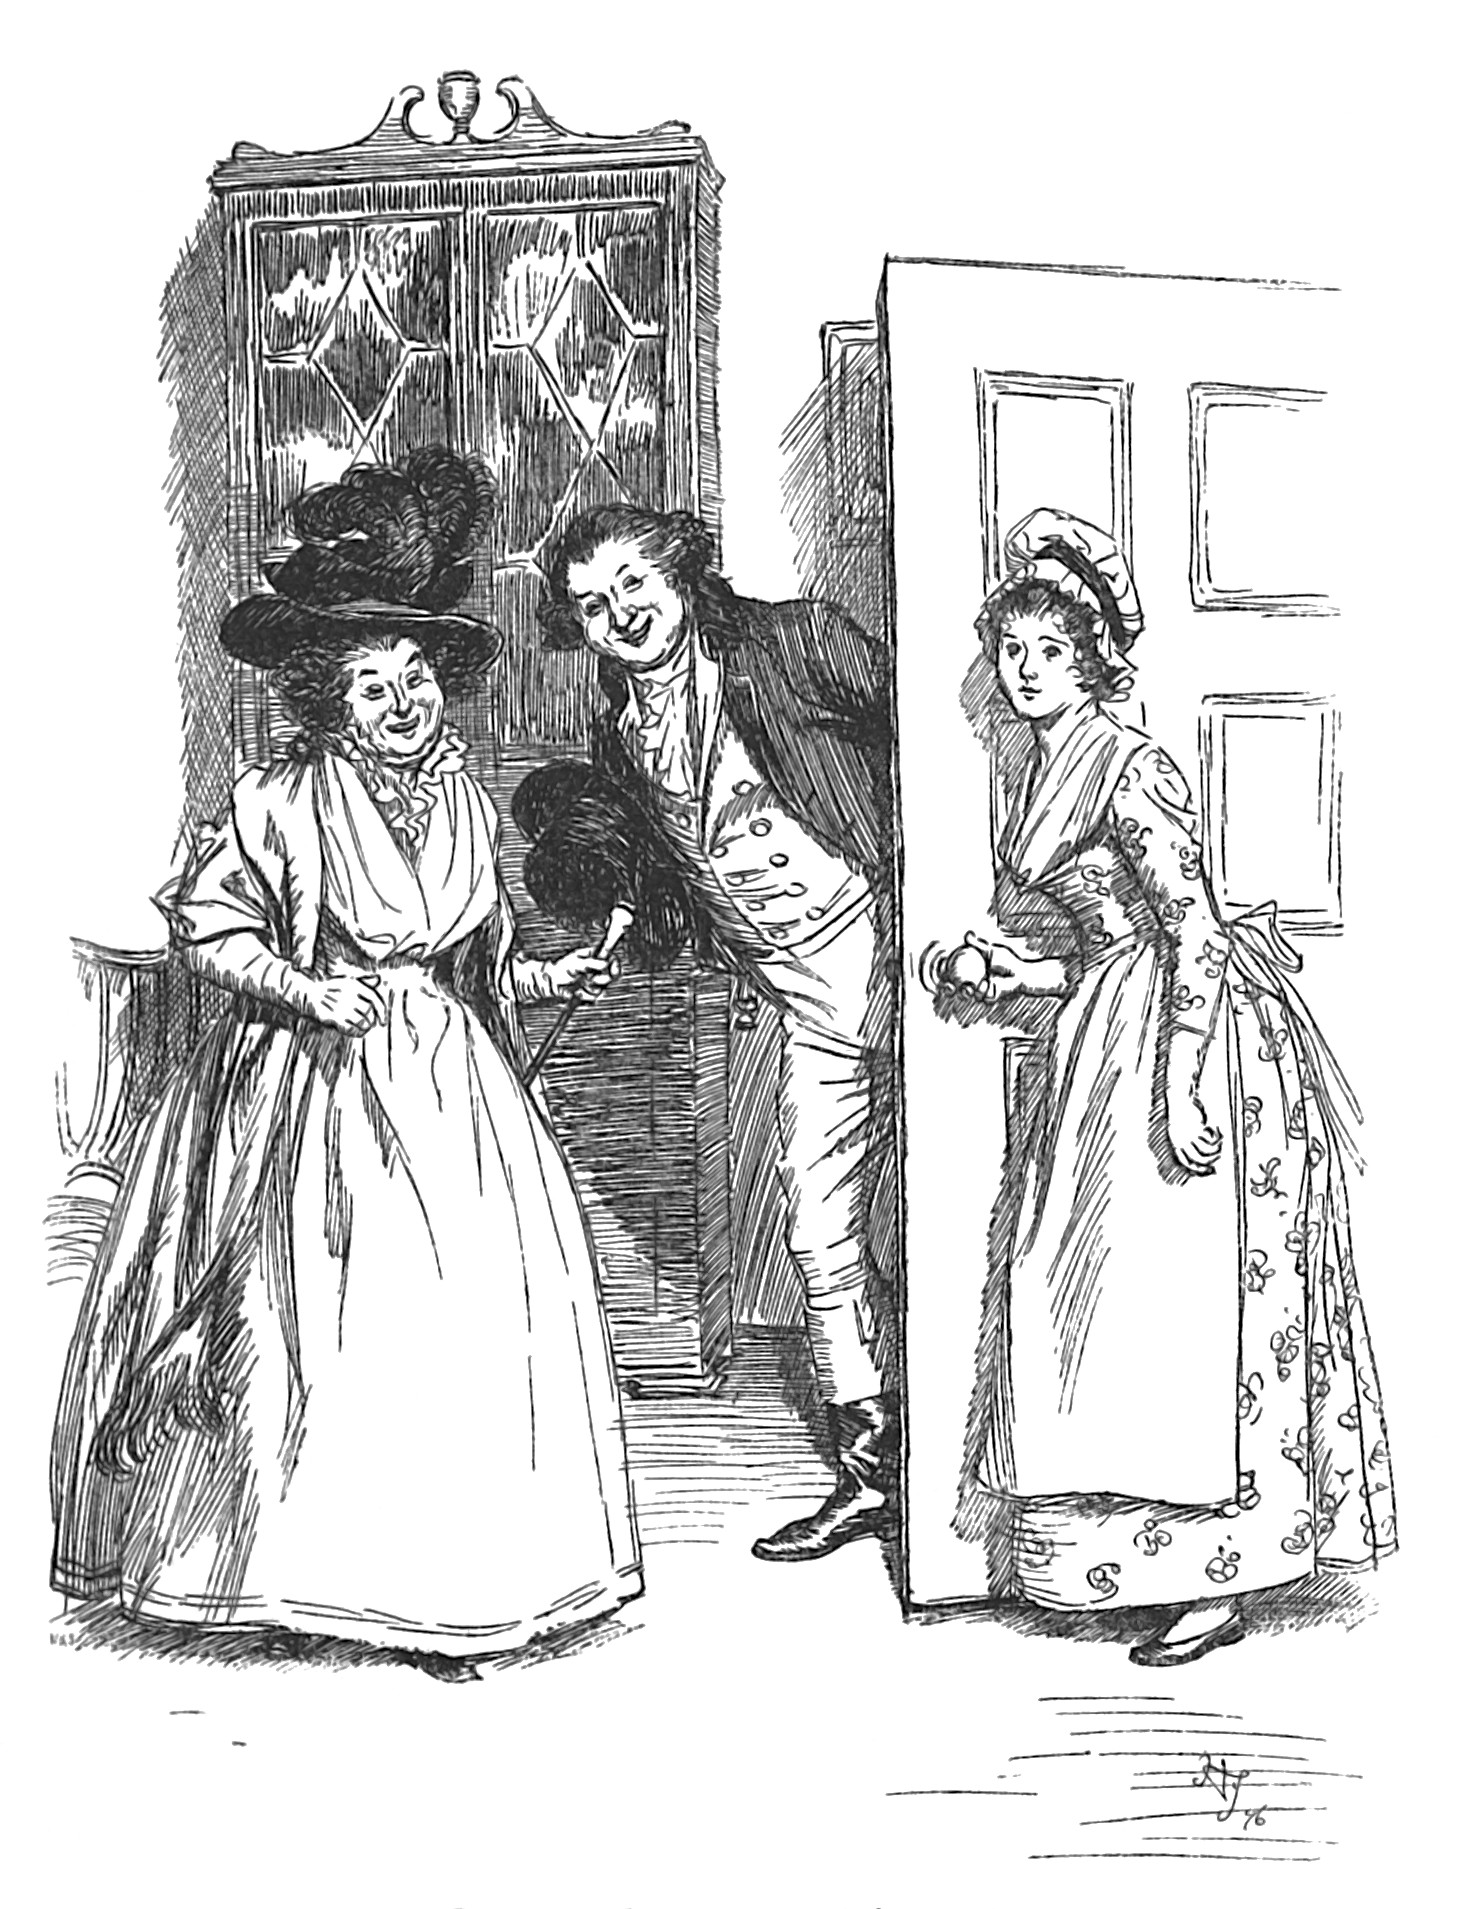
\includegraphics[width=\linewidth]{18guest}
\caption{Came to take a survey of the guest}
\end{figure}

Sir John never came to the Dashwoods without either inviting them to dine at the park the next day, or to drink tea with them that evening. On the present occasion, for the better entertainment of their visitor, towards whose amusement he felt himself bound to contribute, he wished to engage them for both.

»You \textit{must} drink tea with us to night,« said he, »for we shall be quite alone—and tomorrow you must absolutely dine with us, for we shall be a large party.«

Mrs Jennings enforced the necessity. »And who knows but \textit{you} may raise a dance,« said she. »And that will tempt you, Miss Marianne.«

»A dance!« cried Marianne. »Impossible! Who is to dance?«

»Who! why yourselves, and the Careys, and Whitakers to be sure.—What! you thought nobody could dance because a certain person that shall be nameless is gone!«

»I wish with all my soul,« cried Sir John, »that Willoughby were among us again.«

This, and Marianne’s blushing, gave new suspicions to Edward. »And who is Willoughby?« said he, in a low voice, to Miss Dashwood, by whom he was sitting.

She gave him a brief reply. Marianne’s countenance was more communicative. Edward saw enough to comprehend, not only the meaning of others, but such of Marianne’s expressions as had puzzled him before; and when their visitors left them, he went immediately round her, and said, in a whisper, »I have been guessing. Shall I tell you my guess?«

»What do you mean?«

»Shall I tell you?«

»Certainly.«

»Well then; I guess that Mr Willoughby hunts.«

Marianne was surprised and confused, yet she could not help smiling at the quiet archness of his manner, and after a moment’s silence, said,

»Oh, Edward! How can you?—But the time will come I hope...I am sure you will like him.«

»I do not doubt it,« replied he, rather astonished at her earnestness and warmth; for had he not imagined it to be a joke for the good of her acquaintance in general, founded only on a something or a nothing between Mr Willoughby and herself, he would not have ventured to mention it.